\documentclass[12pt]{report}

\usepackage[hidelinks]{hyperref}
\usepackage{graphicx}
\usepackage{cite}
\usepackage[toc,page]{appendix}







\title{Classroom Management Handbook}
\author{Lyron Winderbaum}

\begin{document}

\maketitle

\tableofcontents

\chapter{Introduction}

This document is written as a reference manual of strategies for classroom behaviour management. The goal is that a teacher could consult this document in order to prompt them to think of strategies they could implement in their classroom.

This handbook is organised in chapters. Chapters \ref{chap:preventative}, \ref{chap:supportive} and \ref{chap:corrective} form a list of strategies, each as a section or sub-section therein.
This list is not intended to be comprehensive. These chapters separate strategies into the three broad categories of \cite{Charles2002}: preventive, supportive, and corrective, respectively. The description of each strategy is as minimal as possible. Further discussion of examples and theory are left for later chapters and appendices. Some strategies fall in multiple categories. I will include an entry for a strategy in multiple chapters only if I deem that their use (or purpose) is so different in the different categories context that they warrant consideration as separate strategies. Chapter \ref{chap:video_examples} discusses some of the videos shown in lectures in the context of these strategies, providing some examples of their use in practice. Chapter \ref{chap:theories} introduces a selection of theorists, their theories, and how they relate to the listed strategies.

\textbf{Disclaimer 1:} I've written this document from my perspective, so any statements that are not explicitly referenced to be otherwise are my personal opinion and nothing more.

\textbf{Disclaimer 2:} In some places I might use language such as ``It is wrong to...'', ``You should...'', etc. --- it is important to recognise that every situation comes with it's own intricacies and context and that no such absolute statements can ever be universal.










\chapter{Preventative Strategies}
\label{chap:preventative}

Are preventative in the sense that they describe strategies that can help prevent misbehaviour occurring in the first place. These are by far the most preferable strategies to be using and so should always be the place to start.

\section{Praise}
\label{sec:praise_p}

Praise your students! Some students may never have been praised before, don't underestimate the power it can have. \textbf{Be specific} --- praise some work they have done, or how they self regulated. But most importantly: \textbf{be genuine}, if you are not, your students will know.



\section{Show Interest}
\label{sec:show_interest_p}

Be interested in what is going on in your students lives. This is a natural extension of not assuming and being compassionate (\ref{sec:compassion_s}), but can also lead to learning about what is important to your students and this can allow you to design relevant (\ref{sec:relevance_p}) and interesting (\ref{sec:fun_p}) lessons for them.



\section{Use Names}
\label{sec:use_names_p}

Learn the students names. Use them. Students will appreciate the effort you demonstrated by putting in the work (\ref{sec:show_interest_p}). Similarly to praise (\ref{sec:praise_p}), the impact of this strategy is not to be underestimated.

\textbf{Supportive:} Using names can also be used to reinforce supportive strategies such as praising peers (\ref{sec:acknowledge_good_behaviour_s}) by showing that you are not only noticing a students on-task behaviour, but remembering that specific students name.



\section{Rapport with Students}
\label{sec:rapport_p}

Praise (\ref{sec:praise_p}), using names (\ref{sec:use_names_p}) are both ways of showing interest (\ref{sec:show_interest_p}) in your students. When you do these things you can develop a rapport with the students and that can be a powerful and valuable thing.



\section{Establish Routines and Procedures}
\label{sec:routines_p}

Habit is powerful. If you can instill routines into you class early, you can save yourself alot of headache in the future.

\subsection{Democratic setting of classroom practices}
\label{sec:democratic_setting_of_routines_p}

Discuss classroom practices with students --- give them an opportunity to share their opinions. If they buy into the rules and routines by having influence on deciding what they are, they will have a sense of ownership, and be more likely to follow those rules and routines.

\subsection{Set clear Expectations}
\label{sec:set_clear_expectations_p}

Once the 'rules' of the class have been established, either by you or by democratic process with the class (\ref{sec:democratic_setting_of_routines_p}), ensure to communicate them clearly (\ref{sec:clear_instructions_p}) and enforce them consistently.



\section{Use of Language}
\label{sec:language_p}

The words we choose and the way we speak can have a profound impact on how people perceive us, and students can be particularly sensitive to this.

\begin{itemize}
  \item Use inclusive language --- don't assume (\ref{sec:compassion_s})!
  \item Use clear and concise sentences.
  \item Use appropriate vocabulary.
  \item Articulate well, and at an appropriate volume.
  \item If you have any English as an additional language students, or students with hearing impairments, ensure they have access to the information: 
  \begin{itemize}
    \item Use sign language (if possible), 
    \item Provide translations (if possible), 
    \item Speak slowly and clearly, 
    \item Articulate deliberately,
    \item Do the above without being condescending.
  \end{itemize}
\end{itemize}

\subsection{Clear Instructions}
\label{sec:clear_instructions_p}

It is particularly crucial to be clear when delivering instructions. For verbal instructions,
\begin{itemize}
  \item Be heard: Ensure there is silence before delivering instructions (same as \ref{sec:start_well_p}).
  \item Ensure students have access to all the information they need: If you are asking them to interpret an image, ensure they can see the image, etc. 
  \item Use clear verbs so it is clear what is expected of them (\ref{sec:set_clear_expectations_p}): ``Calculate'', ``Write'', etc.
\end{itemize}

\subsection{Clear Materials}
\label{sec:clear_materials_p}

Delivering instructions clearly equally applies to written instructions, not only verbal instructions (\ref{sec:clear_instructions_p}, \ref{sec:set_clear_expectations_p}). This means using appropriate fonts and vocabulary, etc.



\section{Non-verbals}
\label{sec:non_verbals_p}

Similar to the use of language (\ref{sec:language_p}), non-verbals such as body language, positioning, attitude, facial expressions, etc. have a big impact on how you are perceived. 

\subsection{Enthusiasm}
\label{sec:enthusiasm_p}

The students can tell if you are genuinely enthusiastic about the lesson, about the topic, about seeing them, and enthusiasm is infectious.



\section{Preparation}
\label{sec:preparation_p}

This is an important strategy. If you put in work preparing for your classes, it will pay off both because of the preparation itself, but also because your students will recognise the work you have put in for them, and appreciate it. 

\subsection{Relevance}
\label{sec:relevance_p}

Design material (lessons, activities, etc.) that is relevant to your students lives. If you have some rapport (\ref{sec:rapport_p}) with your students you can ask them what they are interested in and design lessons and activities around their interests.

\subsection{Fun}
\label{sec:fun_p}

Design interesting and fun lessons and activities! Similar to relevance (\ref{sec:relevance_p}) if you have some rapport (\ref{sec:rapport_p}) with your students you could try asking them what they think might be fun and try designing a lesson around that.

\subsection{Variety}
\label{sec:variety_p}

If you do the same kind of activity over and over, it will get boring. Mix it up! Use a variety of approaches and activities both within a class and across classes (\ref{sec:kounin_theory}, \ref{sec:blooms_taxonomy}, \ref{sec:gardner_theory}).

\subsection{Structure}
\label{sec:structure_p}

Design structured lessons. This is vague and broad, but having prepared an appropriate amount of activities and a structure linking them together in a lesson cannot be overstated \ref{sec:kounin_theory}.



\section{Lesson Movement / Momentum}
\label{sec:flow_p}

Having multiple different activities in your lessons is important (\ref{sec:variety_p}, \ref{sec:kounin_theory}). Be aware of transitions between activities. Insist on silence and attention before you deliver instructions for the next activity (\ref{sec:clear_instructions_p}), and work this into a class routine (\ref{sec:routines_p}).

\subsection{Start Well}
\label{sec:start_well_p}

Starting the class represents a big transition: from out-of-class to in-class, and so you should ensure to managed it the same way (\ref{sec:flow_p}). This is a particularly important routine (\ref{sec:routines_p}) to set. One way to manage the start of a lesson in a structured way (\ref{sec:structure_p}) is to use a starter activity. A starter is a short (5-10min) activity that is fun, engaging, and easy, and serves the function of settling the class.




\section{Time Management}
\label{sec:manage_your_time_p}

Reflect on how you have been spending your time in class, and if necessary make adjustments. 



\section{Model Appropriate Behaviors}
\label{sec:model_behaviours_p}

Don't be a hypocrite. If you ask the students to behave a certain way --- adhere to the same standard yourself.


























\chapter{Supportive Strategies}
\label{chap:supportive}

Are for situations when misbehavior is occuring but is not so severe as to require being addressed directly. Supportive strategies aim to encourage and guide students towards adopting more productive and helpful behaviours. 


\section{Praise}
\label{sec:praise_s}

Although praise can be preventative (\ref{sec:praise_p}), it can also be used as a supportive strategy. For students who sometimes meander off task, praising their on-task behaviour can encourage more on-task behaviours.

\subsection{Peer Praise}
\label{sec:peer_praise_s}

One of the strongest forms of praise you can offer a student is that of their peers --- if a student has done something particularly well, encourage their peers to applaud, or similar.
Warning: certain types of students may react badly to this, use with discretion.

\subsection{Praise Peers}
\label{sec:acknowledge_good_behaviour_s}

Misbehaviour motivated by wanting your attention can be managed by praising other on-task students combined with carefully not giving attention to the misbehaviour (\ref{sec:tactical_ignoring_s}).



\section{Be Compassionate}
\label{sec:compassion_s}

You don't know what your students have gone through at home or in their lives. You don't know if their misbehaviour is malicious or is just coming from learnt emotional reactions they have no control over. \textbf{Don't assume}. Train your initial reflex reaction to misbehaviour to be one of compassionate calm. This has the potential to open a door to building rapport (\ref{sec:rapport_p}). It can also help in giving \textbf{genuine} praise (\ref{sec:praise_p}) and showing interest (\ref{sec:show_interest_p}).

This strategy is obviously easier said than done, but it is an important one to keep in the back of your mind as you work on your personal development.



\section{Scaffolding}
\label{sec:scaffolding_s}

If students are losing interest and going off-task as a result of trying, but struggling to complete, a task --- offer to help (scaffold) them in completing the task (\ref{sec:zpd_theory}). If you can give them a sense of success and accomplishment by helping them complete the task, this can encourage future on-task behaviour.



\section{Proximity (``The Whisper Technique'')}
\label{sec:proximity_s}

Proximity can be used as a supportive strategy by using it to deliver help (\ref{sec:scaffolding_s}) privately. Often if you offer help publically (in front of the students classmates) it can be embarrassing for them and they might not be receptive. In contrast, using proximity to deliver aid in a whisper that is not as public can improve the chances that the student will be receptive to the scaffolding.

\textbf{Corrective:} Proximity can also be used to deliver correctives, either a soft corrective simply by placing yourself (the teacher) near the misbehaviour to deter it\footnotemark, or by whispering an admonishment or a direct appeal (\ref{sec:direct_appeal_c}). Warning: Proximity can be very intimidating and can prompt a strong response in students if used in the wrong circumstances or with the wrong student --- use discretion.

\footnotetext{As with most soft correctives the best use would be seamlessly interwoven into your delivery without impacting on the flow of the lesson (\ref{sec:flow_p}, \ref{sec:kounin_theory}).}

\section{Distraction}
\label{sec:distraction_s}

Distract the misbehaving student by giving them something unrelated and interesting to engage their attention.



\section{Tactical Ignoring}
\label{sec:tactical_ignoring_s}

This is the other half of the coin to praising peers (\ref{sec:acknowledge_good_behaviour_s}) when dealing with attention seeking students. You can deliberately ignore off-task behaviour, giving your attention instead to on-task behaviour and the misbehaving students may begin to feel left out, and start to cooperate in an attempt to be included.



\section{Wait Time}
\label{sec:wait_time_s}

Broken sentences --- pause to get attention if students are misbehaving to signal them to stop. This is one of those borderline correctives, also called ``Canter's ``Broken Record'''' in Figure~\ref{fig:correctiveHierarchy}.


\section{Challenge Students}
\label{sec:challenge_s}

Particularly if you suspect the misbehaviour is motivated from boredom, issue a challenge to the misbehaviours to complete some task --- preferably a relevant and engaging task (\ref{sec:relevance_p}, \ref{sec:fun_p}) that will challenge them. 



\section{Use Humour to Depotentiate}
\label{sec:humour_s}

Is a students misbehaviour has led to confrontation or tension in the classroom, try using humour to depotentiate the situation.

























\chapter{Corrective Strategies}
\label{chap:corrective}

Are for the times when students misbehave to a point that their misbehaviour must be addressed directly and can no longer be managed by supportive strategies alone. The central thinking when implementing a corrective should always be to avoid escalation. The harsher the corrective used, the more likely it is to result in escalation, and so it is always preferable to use the softest corrective possible that manages the behaviour. See Figure~\ref{fig:correctiveHierarchy}.

It is also important to note the special case of chronic misbehaviour --- in this case it is particularly important to try to understand the underlying cause of the misbehaviour, for which Dreikurs' social discipline model (\ref{sec:dreikur_theory}) can be particularly helpful. Hence I have incorporated my discussion of strategies for managing chronic misbehaviour into section \ref{sec:dreikur_theory}.


\begin{figure}[p]
\begin{center}
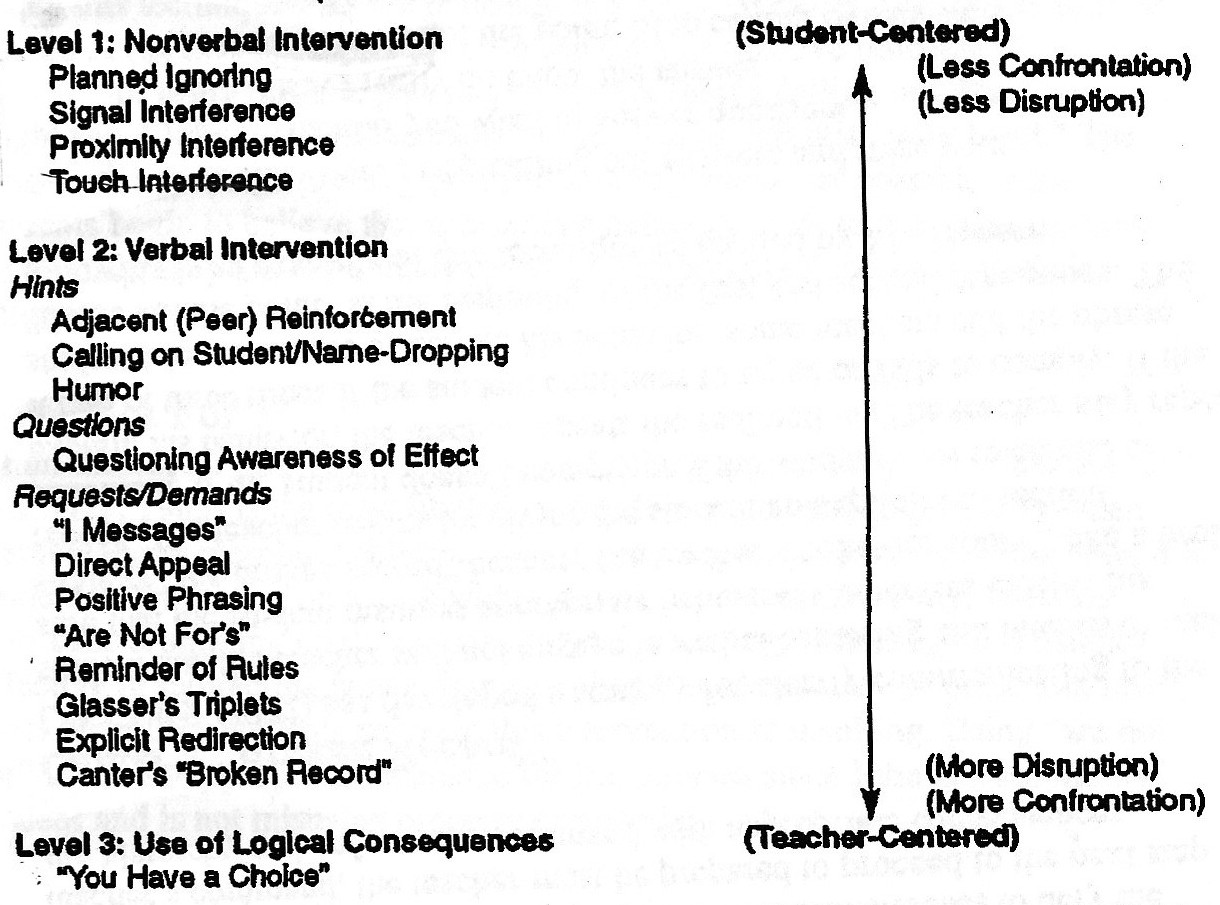
\includegraphics{./images/correctiveHierarchy.jpg}
\end{center}
\caption{Hierarchy of Management Intervention Diagram \cite{Levin2005} showing a list of corrective strategies, ranked in increasing order of harshness. Some of these are not applicable (such as touch), and others have already been covered as supportive strategies such as "Planned Ignoring" (\ref{sec:tactical_ignoring_s}), "Proxomity Interference" (\ref{sec:proximity_s}), "(Peer) Reinforcement" (\ref{sec:peer_praise_s}), and "Humour" (\ref{sec:humour_s}), as there is a grey area betwene supportive and soft corrective strategies. \label{fig:correctiveHierarchy}}
\end{figure}


\section{Eye Contact}
\label{sec:eye_contact_c}

Catch the misbehaving students' eye from across the room and hold their gaze for a moment\footnotemark. 



\section{Calling on Student}
\label{sec:use_names_c}

Call out the misbehaving student by name\footnotemark[\value{footnote}].



\footnotetext{As with most soft correctives the best use would be seamlessly interwoven into your delivery without impacting on the flow of the lesson (\ref{sec:flow_p}, \ref{sec:kounin_theory}).}



\section{Questioning Awareness of Effect}
\label{sec:questioning_c}

Ask the misbehaving student if they are aware of the effect their behaviour is having on the class or surrounding students\footnotemark.



\section{Gordons I-Messages}
\label{sec:i_messages_c}

Gordon (\ref{sec:gordon_theory}) suggested a three step process for initiating a conversation with a student in a non-confrontational\footnotemark[\value{footnote}] way (at least that is the intention!)  about behaviour the teacher is unhappy with:
\begin{itemize}
  \item Describe the disruptive behaviour.
  \item Describe the effect on the teacher and/ or other students.
  \item Describe your feelings about the behaviour.
\end{itemize}



\section{Reminder of Rules}
\label{sec:reminder_c}

Remind the student, by name (\ref{sec:use_names_c}), of the rule they are in violation of. Note that these rules should have already been clearly (\ref{sec:language_p}) set out previously (\ref{sec:routines_p}) --- that they are breaking\footnotemark[\value{footnote}].



\section{Direct Appeal}
\label{sec:direct_appeal_c}

Tell the student, by name (\ref{sec:use_names_c}), to stop the misbehaviour. Note: do not ask or use "please", you are giving a directive\footnotemark[\value{footnote}].



\section{Glassers Triplets}

Are three questions that can be posed to a student to answer:
\begin{itemize}
  \item What are you doing?
  \item Is that against the rules?
  \item What should you be doing instead?
\end{itemize}
If the student is being uncooperative, instead of engaging in a confrontation 
you should simply state the answers to these questions and move on\footnotemark[\value{footnote}].



\section{Private Talk}
\label{sec:private_talk_c}

Arrange for a time out of class to talk with the student or students. Often it might be easiest to ask them to stay after class\footnotemark[\value{footnote}]. This would be one of my preferred correctives, should a strong corrective be needed. 

\footnotetext{Having some rapport (\ref{sec:rapport_p}) with the student can greatly increse the chances of a successful outcome from stronger corrective strategies such as these.}


\section{Give Choice}
\label{sec:give_choice_c}

Give the misbehaving student a choice: either stop the misbehaviour, or suffer a consequence. 

\section{Apply Sanctions}
\label{sec:sanctions_c}

If the student has:
\begin{itemize}
  \item been given a choice (\ref{sec:give_choice_c}) and chosen not to stop the misbehaviour, or 
  \item broken an established rule (\ref{sec:routines_p}) either defined by you, the school, or by the class (\ref{sec:democratic_setting_of_routines_p}), 
\end{itemize}
then you must deliver the consequence, which could be anywhere from staying back after class, having a chat with you (\ref{sec:private_talk_c}), being ejected from the class, detention, or even exclusion or suspension.














\chapter{Video Examples}
\label{chap:video_examples}

Preparation (VIDEO: Praise and Preparation, Amy)

 Amy is a good example of structure this (VIDEO REFERENCE).

Non-verbals such as being happy to see the students (VIDEO: Talk too much).
A fantastic example of non-verbals this is simply being (genuinely) happy to see the students.
(VIDEO REFERENCE). Warning: Similar to with praise (\ref{sec:praise_p}), being genuine is crucial in this example --- if you are not genuine the students will be able to tell.



 (VIDEO: Manage that lesson (chemistry year 8)


\section{Praise and Preparation (Teaching with Bayley --- Amy)}

\href{https://youtu.be/KkXRjrSsMQg}{Link to video}


% \section{Too Much Talk (Teaching with Bayley --- }
% 
% \href{http://archive.teachfind.com/ttv/www.teachers.tv/videos/too-much-talk.html}{Link to video}



\section{Manage that Class (Teaching with Bayley --- Jenny)}

\href{http://archive.teachfind.com/ttv/www.teachers.tv/videos/manage-that-class-year-8-friday.html}{Link to video}



% \section{The Need for Structure (Teaching with Bayley --- )}
% 
% \href{http://archive.teachfind.com/ttv/www.teachers.tv/videos/the-need-for-structure.html}{Link to video}




\section{Argument Tennis (Phil Beadle)}

\href{https://www.youtube.com/watch?v=zr2xdjQPH4I (Links to an external site.)Links to an external site.}{Link to video}




% \section{Love 'em or loathe 'em (Teaching with Bayley --- )}
% 
% \href{https://www.youtube.com/watch?v=YUo61Uj4Cmg (Links to an external site.)}{Link to video}





\section{Attension Seekers (Teaching with Bayley --- French Teacher)}

\href{https://www.youtube.com/watch?v=pXhtwDK4oHw}{Link to video}





% \section{Underachieving Boys ( )}
% 
% \href{https://www.youtube.com/watch?v=42p59Upj_M4 (Links to an external site.)}{Link to video}
% 
% 
% 
% \section{Key Instructions ( )}
% 
% \href{https://www.youtube.com/watch?v=FP7GyfGKamQ}{Link to video}




\section{Chatty Girls (Teaching with Bayley --- Maths Class)}

\href{https://www.youtube.com/watch?v=Q3OxKAxpOdo}{Link to video}





\section{Tough Love (David Torn)}

\href{https://www.youtube.com/watch?v=ec0v4kzYkCY}{Link to video}






\section{Underachieving Boys: The Play's The Thing.}

\href{https://www.youtube.com/watch?v=9196qkVWaLw}{Link to video}













\chapter{Theories and Theorists}
\label{chap:theories}


\section{Blooms Taxonomy}
\label{sec:blooms_taxonomy}

% \begin{figure}[h]
% \begin{center}
% \includegraphics{./images/circle.gif}
% \end{center}
% \caption{Blooms Revised Taxonomy Wheel \label{fig:bloomsTaxonomy}}
% \end{figure}



\section{Garder's Multiple Intelligences}
\label{sec:gardner_theory}



\section{Thomas Gordon}
\label{sec:gordon_theory}

The approach of Thomas Gordon is centred on "the importance of developing meaningful mutually beneficial relationships" (\href{https://en.wikibooks.org/wiki/Classroom_Management_Theorists_and_Theories/Thomas_Gordon}{wiki page}). Gordon claims that in relationships each participant (in this case students and teachers) bring their own values and needs and these will disagree and result in conflict. Gordon suggests that to resolve such conflicts the first step is to identify who "owns" the problem --- that is, which is the disgruntled party. Then:
\begin{itemize}
  \item If the student "owns" the problem, the teacher should engage in "active listening" --- that is they should listen to the students grevance and genuinely try to understand and empathise with their frustrations (\ref{sec:show_interest_p}, \ref{sec:compassion_s}, \ref{sec:non_verbals_p}).
  \item If the teacher "owns" the problem, then they should use an "I-message" (\ref{sec:i_messages_c}) to initiate a conversation in a non-confrontational way.
\end{itemize}
Finally, the object in Gordons framework is to acheive a solution in which both parties have contributed and feel invested in, similar in principle to the buy-in discussed in \ref{sec:democratic_setting_of_routines_p}.


\section{Vygotsky's Zone of Proximal Development (ZPD)}
\label{sec:zpd_theory}


Amongst other things, Vygotsky proposed the ZPD model for learning. The ZPD model claims that all learning occurs in the ZPD, which is defined as the set of tasks and activities or concepts that the students cannot complete or understand without help, but with help can. This is the essence of the concept behind scaffolding (\ref{sec:scaffolding}). If students are given tasks so difficult they cannot complete them successfully even with help from the teacher, or they are given tasks so easy they can complete them easily on their own, they will not learn anything, and they will likely quickly lose interest in the lesson, become bored, and misbehave. Only if they are given tasks of just the right level of difficulty, and are given assistance in completing those tasks, will they learn and engage.



\section{Jacob Kounin}
\label{sec:kounin_theory}

Kounin suggests that transitioning from activity to activity during a lesson is important in order to maintain engagement (\ref{sec:variety_p}) and called this ``Lesson Movement'' (\ref{sec:kounin_theory}). These transitions need to be managed well however as they are often when students will become restless, which can result in losing ``momentum''. Managing transitons is a difficult skill to master, and requires a certain ``withitness'' (a term coined by Kounin  --- \ref{sec:kounin_theory}). ``Withitness'' involves being constantly aware of the class to a level of detail that you can tell when the class is about to become restless and intercde before that happens. Developing ``withitness'' takes time and experience, but managing transitions can also be made less difficult through good preparation (\ref{sec:prepartation}) with plenty of structure (\ref{sec:structure}), and the delivery of clear instructions (\ref{sec:clear_instructions_p}).

Jacob Kounin wrote alot about the effect a teacher can have on misbehaviour in their class through mostly preparatory techniques (\ref{sec:preparation_p}) such as structuring lessons well (\ref{sec:structure_p}), with a focus on what he refered to as "Lesson Movement" (\ref{sec:flow_p}). Kounin is the one who coined the term "withitness".

Also noticed the "Ripple Effect", and sugggested a broad categorisation of attributes a teacher should focus on developing in their lessons: Withitness, Overlapping, Momentum, Smoothness and Group Alerting. For more detail refer to \href{http://universityofhullscitts.org.uk/scitts/site/pt/behaviour/kounin.html}{this website}.

\section{Dreikurs' Social Discipline Model (in the context of chronic misbehaviour management)}
\label{sec:dreikur_theory}

Very breifly, Dreikurs' Social Discipline Model can be used to diagnose and approach chronic misbehaviour by first identifying the goal of the behaviour, which is usually one of:
\begin{itemize}
  \item Attrating Attention,
  \item Power,
  \item Revenge, or
  \item Escape by Withdrawl.
\end{itemize}
What the goal of the behaviour is can often be diagnosed by observing the effect the behaviour has on the teacher. If the teacher feels:
\begin{itemize}
  \item Minor annoyance and frustration, then the goal was likely attention seeking.
  \item Personally challenged, then the goal was likely power. 
  \item Deeply hurt, then the goal was likely revenge.
  \item Like giving up, then the goal was likely escape by withdrawl.
\end{itemize}
The most common goals of chronic misbehaviour are attracting attention, and escape by withdrawl, and there are two broad approaches to addressing chronic misbehaviour which can be roughly matched against these two goals:
\begin{itemize}
  \item Relationship Building (to address mostly attention seeking behaviours): through building rapport (\ref{sec:rapport_p}) and having private conversations (\ref{sec:private_talk_c}) with the student, often acceptable behaviours can be negatioated where both the teachers and the students needs are being met.
  \item Breaking the cycle of discouragement (to address mostly escape by withdrawl behaviours): through scaffolding (\ref{sec:scaffolding}), careful design of lessons and praise (\ref{praise_s}), the student can be given a feeling of success which can sometimes break through their cycle of discouragement.
\end{itemize}
  








\begin{appendices}

\chapter{Elaboration on Stategies with Examples}

\section{Manage your Time}
Examplees of time-management --- have you been spending all your time speaking to the same students, are there some that have not had a chance to speak to you or get your attention? Have you been spending alot of time in class doing things that could be done beforehand (\ref{sec:preparation_p}), like writing on the whiteboard for example? Are these important? If the answer to any of these leading questions is yes, considering managing your time differently --- explain that you will only spend a certain amount of time with each student s

\section{One-on-One}

In that setting, away from the social pressures of their peers, you may be able to have a more productive conversation about their behaviour, maybe learn where it originates from,




\chapter{More Theories and Theorists}


\section{Maslow's Hierarchy of Needs}


\section{Glasser's Choice Theory}


\section{Piaget's Developmental Stages}



\section{Skinners' Operant Conditioning}

\section{Cognititive Load Theory}

Cognitive Load Theory, originally attributed to (Sweller?), is a learning model in which it is hypothesises that the number of new or unfamiliar concepts that can be held in working memory at any given time is limited. The practical consequences of this are similar to those of ZPD, in that the amount of work, the number of new concepts, provided to students need to be metered out at an appropriate rate. If too much information is provided all at once, the students will go into cognitive (over-)load, and will simply zone out --- and likely misbehave.


\end{appendices}

\bibliography{references}{}
\bibliographystyle{apalike}


\end{document}